\subsection{Zonificación}
\label{subsec:cap4-zonificacion}
Cada entorno puede contar con factores que lo hagan más o menos apto para el desarrollo,
mortalidad, alimentación, disperción, y reproducción de individuos. En esta sección, con el fin de
simplificar ciertos aspectos muy especificos que se encuentran fuera del alcance de este trabajo,
realizaremos ciertas hipótesis generales, justificadas para nuestro caso de aplicación, pero puede
requerir una revisión en el caso general. Estas hipotesis son, los valores observados en un
conjuto de puntos de control, pertenecientes a una zona, permiten la caracterización de dicha zona como más o menos apta para desarrollo, mortalidad, alimentación, disperción, y reproducción de
individuos. Tambien consideramos que el tamaño de la zona, y por ende la cantidad de puntos de
control que pertenecena ella, influye en la caracterización de las zonas.

La zonificación surge ante necesidad de dividir el espacio de estudio de una forma más granular,
para identificar a los individuos que pertenecen a zonas aptas y los que no. Los puntos de control
distribuidos en un área de estudio nos permite estimar cuales zonas los niveles de riesgo e
infestación correspondiente a la abundacia de larvas por litro que se pueden observar.

\begin{table} [H]
    \begin{minipage}{\textwidth}
\begin{center}
    \caption{\label{tab:cap4-puntaje-zona} Clasificación de las zonas de acuerdo a la densidad de larvas por litro.}
    \begin{tabular}{p{3cm} c c c c}
        \\
                     & Mínimo$^a$ & Máximo$^a$ & Hembras     & Hembras$^c$ \\
        Tipo de zona & $u(x,y)$   & $u(x,y)$   & Adultas$^b$ & Reproductivas$^c$ \\
        \hline
        \hline\\
        Pésima  & 0  & 19 & 8  & 5 \\
        Mala    & 20 & 35 & 15 & 10\\
        Regular & 36 & 51 & 22 & 15\\
        Buena   & 52 & 69 & 30 & 20\\
        Óptima  & 70 & --$^d$ & --$^d$ & --$^d$\\
    \end{tabular}
    \footnotetext[1]{Rango mínimo y máximo de $u(x,y)$ permitido para el tipo de zona.}
    \footnotetext[2]{Cantidad máxima de hembras adultas, al final del periodo de desarrollo.}
    \footnotetext[3]{Cantidad de hembras adultas con capacidad de oviponer.}
    \footnotetext[4]{No se estableció un límite superior para las zonas óptimas. }
\end{center}
    \end{minipage}
\end{table}

En la \tabref{tab:cap4-puntaje-zona} se puden observar los rangos definidos para cada tipo de
zona, en donde $u(x,y)$ es la densidad relativa, en un radio, $r$. El valor de $u(x,y)$ es
estimado, a partir de los valores conocidos de los puntos de control, mediante el método de
interpolación definido por ecuación \eqref{eq:interpolacion-idw} (\figref{fig:cap4-zonficiacion}).
Los límites para las zonas fueron determinados clasificando los valores, de las hembras
reproductivas en, grupos múltiplos de cinco. No se estableció un límite superior para las zonas
óptimas debido a que los valores mayores a el mínimo establecido, 70 larvas por litro, pertenecen
a la misma categoría.

\begin{figure}
\centering
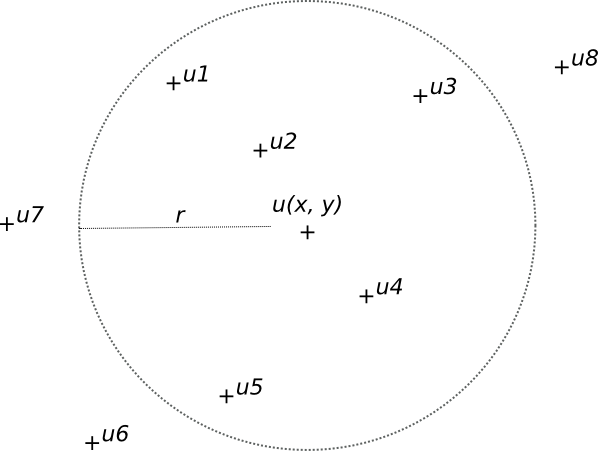
\includegraphics[width=0.6\textwidth]{capitulo-4/graphics/zonificacion.png}
\caption{\label{fig:cap4-zonficiacion} Relación entre el radio $r$, el valor de $u(x,y)$ a estimar y los valores conocidos.}
\end{figure}

El tamaño del radio, $r$, es un parametro ajustable del modelo, mientras más grande sea el tamaño
del radio, más puntos serán incluidos para el cálculo, lo que gerará que las zonas tiendan a ser
similares. Para el calculo de las hembras adultas y reproductivas para la clasificación de las
zonas se tuvieron en cuenta que, solo el $50$ \% de las larvas observadas son hembras
\cite{otero2006stochastic, manrique1998desarrollo}, la temperatura media utilizada es de 25
\textcelsius \cite{website:mspbsHistoria2014}, la mortalidad díaria natural bajo optimas
condiciones,a 25 \textcelsius, es de 0,01 según \eqref{eq:mortalidad-natural-larvas}, la tasa de
desarrollo, a 25 \textcelsius, de la larva hasta su emergencia a adulto es de $11.57$ días
\cite{rueda1990temperature}, y que el $32.10$ \% de las hembras adultas no ovipone
\citep{osoriopontificia}.
